\chapter{基于循环机制的运动特征增强视频显著性检测网络}
\renewcommand{\leftmark}{第四章\quad 基于循环机制的运动特征增强视频显著性检测网络}

\section{引言}
在前面的两个章节中,本文详细介绍两个本文提出的两种视频显著性检测的方案,分别是级联深度网络(SCNN)和注意力时空特征融合网(STAN)。其中SCNN主要针对的训练数据不足,提出一个并行迭代弱监督策略。而STAN是针对的是SCNN静态与运动特征的融合方式存在问题,提出了一种新型的双流子网络结构,并采用注意力机制融合子网,运动精炼模块生成的不同类型的特征。总的来说,SCNN和STAN都是从不同角度去解决视频显著性领域存在的问题,同时也取得了有竞争力的结果。

虽然研究视频显著性目标检测的人员相对较少,但是随着时间的推移许多更为直接有效而且更为实用的方法也被陆续被提出,其中比较好的方法有FGRNE\cite{li2018flow}、PDB\cite{song2018pyramid}、SSAV\cite{Fan_2019_CVPR}。从整体上来总结,近期提出的方法是从分布到端到端的发展趋势,并且这些方法开始逐渐地把视频显著性目标检测与视频目标分割方法同一起来,形成一套通用的方法。为了研究出更好的视频显著性方法,本章需要详细介绍一下上述三个方法。

首先是FGRNE方法,该方法发表于2018初,主要是思路仍深度网络与光流图进行配合。由于光流图在运动目标捕捉上有高准确率,因此FGRNE没有放弃使用这一运动特征。也正是没有放弃使用这一特征,其深度网络不是严格意义上的端到端网络。在使用该深度网络之前,光流图需要预先得到,而且由于光流图的提取需要大量的时间,从而影响整个显著性检测过程的处理时间。虽然,FGRNE方法引入光流影响了速度,但是它的网络结构结合了DSS的短连接和LSTM运动模块,可以充分地提炼显著性特征,进而生成优质的显著图。因此,其结果相比于之前提出的方法有质的飞跃,在某些指标上甚至可以提高好几个百分点。

然后是PDB方法,此方法即为严格意义上的端到端方法。由于摆脱了对光流图的依赖,PDB网络是仅输入原始的视频帧,之后直接生产高质量的显著图。PDB能产生比FGRNE还准确显著图的原因,本文认为有两点,其一是合理的静态特征提取器。该提取器主要由两部分组成,第一部分是基础网络——ResNet50。在PDB之前的深度学习方法主要使用的基础网络是VGGNet,相比于ResNet50,VGGNet的层数稍浅,网络泛化能力也稍弱。而引入了ResNet50后,PDB可以提取到鲁棒性更高的高层语义特征。第二部分是修改自DeeplabV3\cite{chen2017rethinking}的金字塔级分层膨胀卷积。我们知道DeeplabV3在分割方面有这很大的优势,其Atrous Spatial Pyramid Pooling(ASPP)结构可以通过多重感受野抓取到不同等级的深度特征。PDB是在其基础之上,把感受野进一步加大,能在做卷积滑动时有更大的范围,进而得到更为多样的特征图。PDB的第二个优势是其运动特征的精炼。PDB通过双向多级膨胀ConvLSTM来提取运动特征,其双向结构可以充分利用帧间关系,再加上膨胀卷积增加感受野,在原有静态特征的基础之上提取到了多尺度运动信息,这种多类型的时空特征非常有利于显著图的生成。最终,PDB的结果可以在FGRNE之上又提高了几个百分点,而且由于没有使用光流图,其端到端的结构使其运算速度可以达到20帧每秒。

最后是SSAV方法,相比于上述两个方法,SSAV在方法上创新较少,其主要是对之前视频显著性检测方法做了一个总结与归纳并且建立了一个超大型的视频显著性检测数据库。在其建立数据库的过程中,他们发现在连续视频中,运动目标可能随着时间的变化而变化。在方法上,他们以PDB网络为基础,把数据集中用眼动仪标定的人眼注意力标签引入网络,提出了一种新型的ConvLSTM结构(saliency shift-aware convLSTM)来捕捉随视频改变的显著目标。因此,其最终结果在某些数据集上比PDB的效果还好。而且,SSAV最大的贡献是一个大型的benchmark,里面尽可能收录了从2010年以来的所有视频显著性方法,并且分别在8个数据集上做了评价。

综上所述,视频显著性检测的发展趋势是从分步骤处理到端到端网络,运动特征也摆脱了光流的限制,可以直接使用视频序列通过网络训练得到,而且实验效果也越来越好,甚至在一些数据集中它们的结果已经与真值相差无几。举个例子,PDB在MCL数据上的平均错误率(MAE)可以低至0.021,可以通俗了理解为100个像素中只有两个像素有错误。而SSAV在ViSal数据集中的平均错误率可达到0.020。相比于FGRNE、PDB、SSAV,本文提出的SCNN和STAN也使用到的光流图,因此也降低的整个方法的处理过程。虽然在模型上各有可取之处,但是在特征精炼上,上述三种更为合理。因此,为了超过上述方法,在如此高的实验结果中再进行提升需要更为精细的分析。

本文在实验的过程中,通过可视化深度网络中的运动精炼模块ConvLSTM生成的特征图,我们有了一些发现。在很少了一些视频序列中,序列中某几个连续帧的特征图存在明显的跳变,如图\ref{pull_figures}所示,我们可以看到相差很小的连续两帧(图\ref{pull_figures}(a)),其最终的显著图(图\ref{pull_figures}(c))相差很大,即有一个明显的跳变。然而,通过观察两帧的深度特征图(图\ref{pull_figures}(b)),我们可以发现显著目标都已经被检测到(黄色部分),但是通过右边的颜色条可以看出,后一帧的特征数值较低,而且大多数特征值都小于零,这一个特征图被Sigmoid函数激活后,其值会趋近于零,所以表现出来的显著图也就不能显示对应的显著目标了。从中我们可以看出只使用ConvLSTM来提炼运动信息仍有不足,可以采用更为合理的结构来进一步增强运动特征。

发现这一现象后,本文就开始尝试解决这一问题。由于一个视频序列中可能只有某几帧存在这样的问题,那么问题帧之前的视频帧是可以正常检测到的。并且特征图中的数值也相对较大(图\ref{pull_figures}(b)红色区域可以看出),所以本文的方案即为采用以前帧引导当前帧的意思,并结合ConvLSTM可以精炼运动的特点,提出了一个循环运动特征增加的网络结构。该结构主要采用两种方式来增加运动特征。第一,稠密循环运动特征增强,即把通过一个循环体把ConvLSTM得到的特征按时间顺序依次向前融合,令当前帧的特征值变大。第二,显著图先验引导,即把前面多帧的生成显著图作为先验,然后合并到特征图上,引导特征图有方向性的学习显著特征。这两个结构会在本章后面的内容中详细介绍和通过实验做具体分析。

综上所述,本章详细地分析了最近的视频显著性目标检测方法,同时在自己实验的过程中发现个别序列中存在显著性检测在视频中段突然失败,进一步研究发现是ConvLSTM生成的特征图中的像素值偏低。本文为了解决这一个问题提出一个循环运动增强模块,该模块可以利用帧间关系,通过迭代不断地增强运动特征,从而解决视频中段目标检测失败的问题。在实验方面,本章提出的方法取得了有竞争力的结果,在几个通用数据集都不小的提高,甚至超过现阶段最为准确的两个方法PDB和SSAV。同时,本章也无监督视频目标分割数据集上做了验证,证明本文的方法在无监督视频分割上也是有效的,具体的分析将会在本章的实验部分具体介绍。

本章的内容安排如下:首先是引言,分析了最近最好的三个方法的优势和本文通过自身实验发现的问题,并以此为契机提出了自己的方法来解决这一问题。其次是相关网络结构的介绍,本文需要先介绍本章利用到的网络结构,以便之后更为方便地描述本章提出的方法。接着是方法描述,详细介绍了本章提出的方法。之后是详细的实验分析,包括两部分实验,其一是视频显著性目标检测的实验评价;还有就是无监督视频目标分割的实验评价。在本章的最后会有一个小结来总结本章提出的方法。
\begin{figure*}
%\vspace{-100pt}
\center
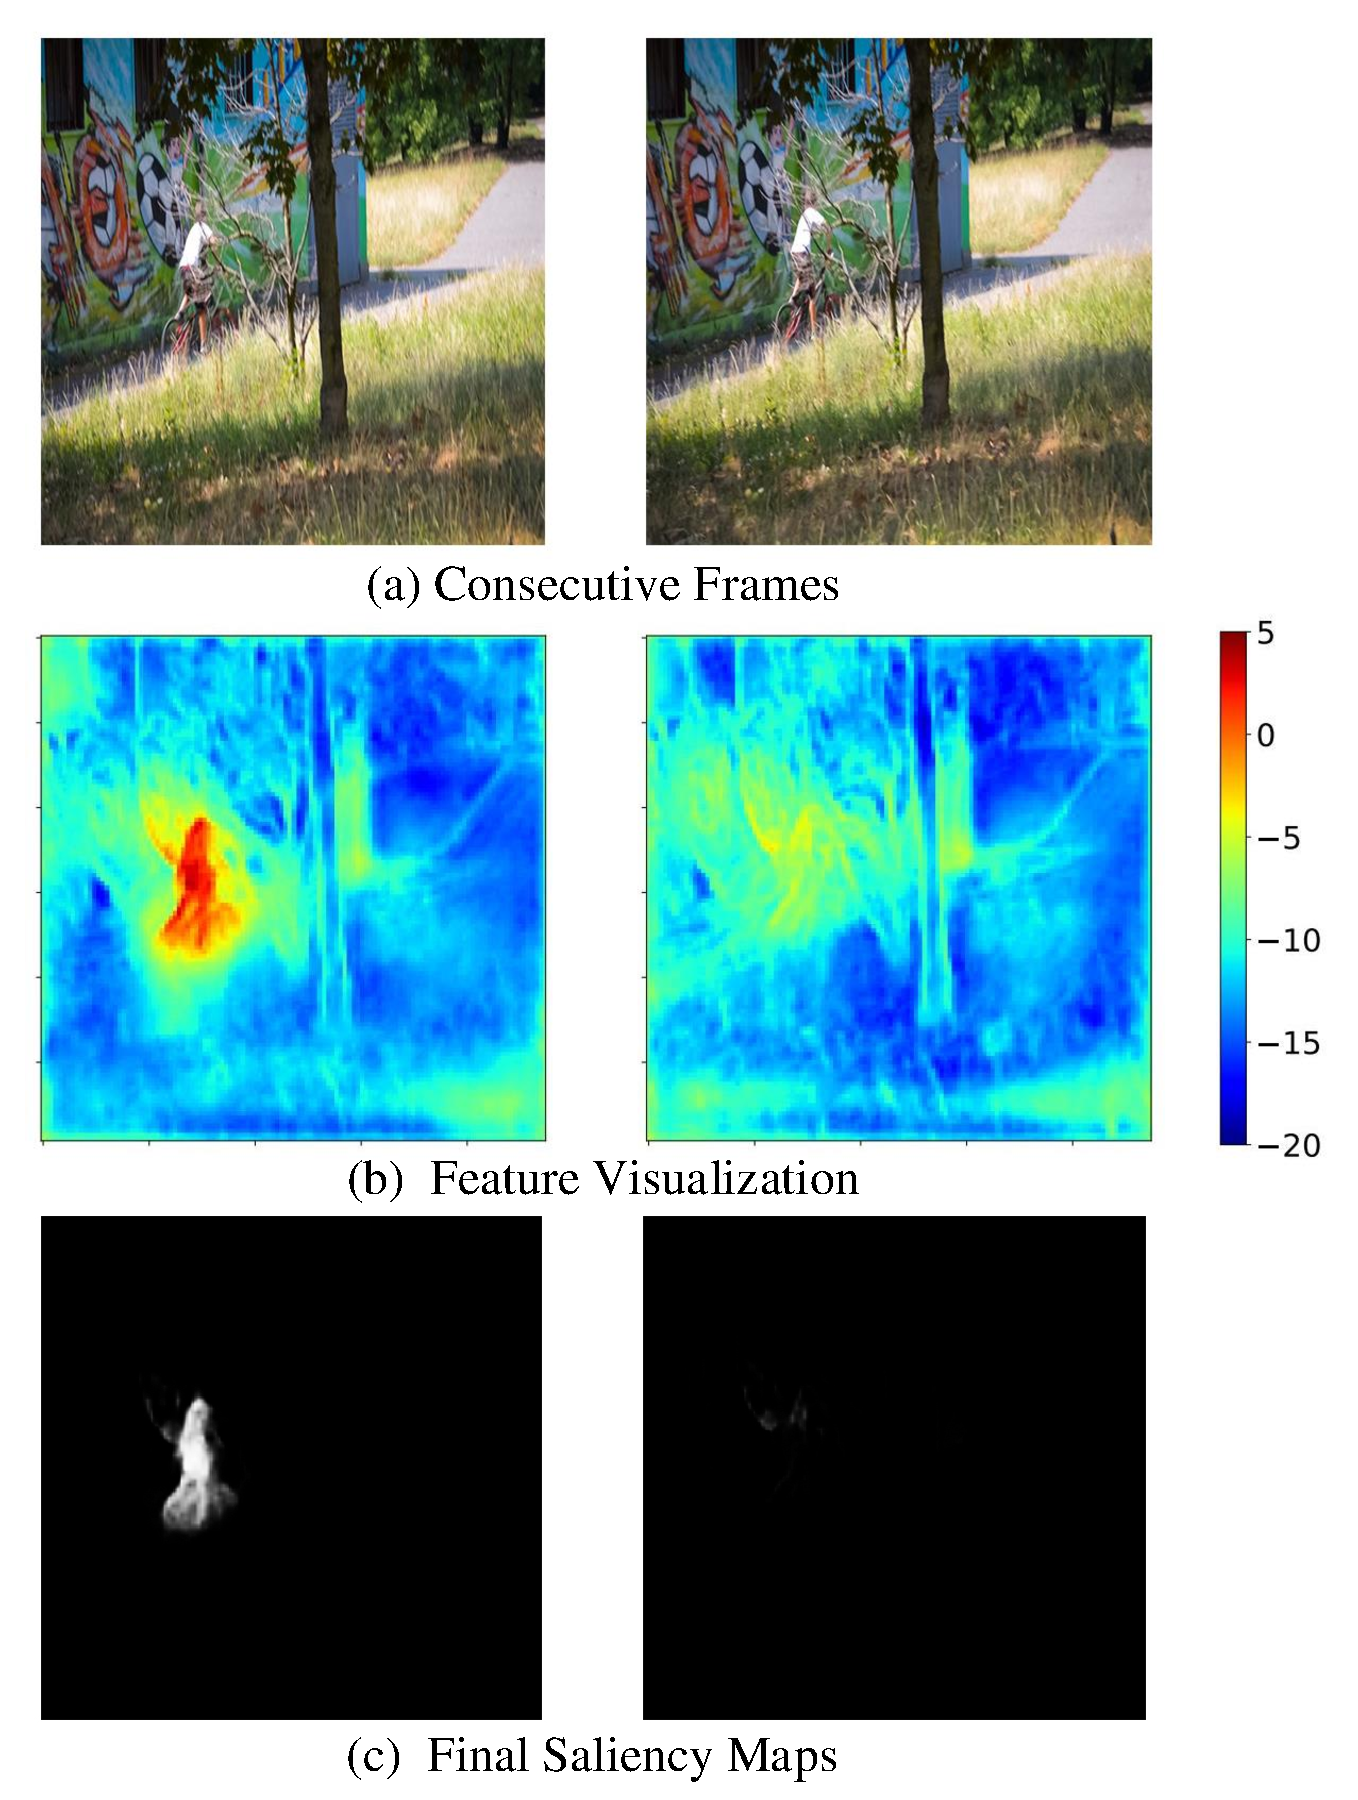
\includegraphics[width=0.8\textwidth]{figures/pull_figures_c4}
\caption{Saliency maps by different configurations of the network. From left to right, they are saliency maps by only.}
\label{pull_figures}
%\vspace{-5pt}
\end{figure*}

\section{相关的深度网络模块}
本文提出的运动特征增强网络(MEN)是一个端到端的网络,本文是在一个基础网络之上加入运动特征增加模块来实现视频显著性检测的。同时,我们可以把基础网络看成一个特征提取器,因此基础网络的结构对最终显著性估计有着重要的贡献。在本节中,本文先介绍两个基础网络中最为重要的模块,ResNeXt结构和Atrous Spatial Pyramid Pooling(ASPP)结构。

\subsection{ResNeXt网络结构}

\begin{figure*}
%\vspace{-100pt}
\center
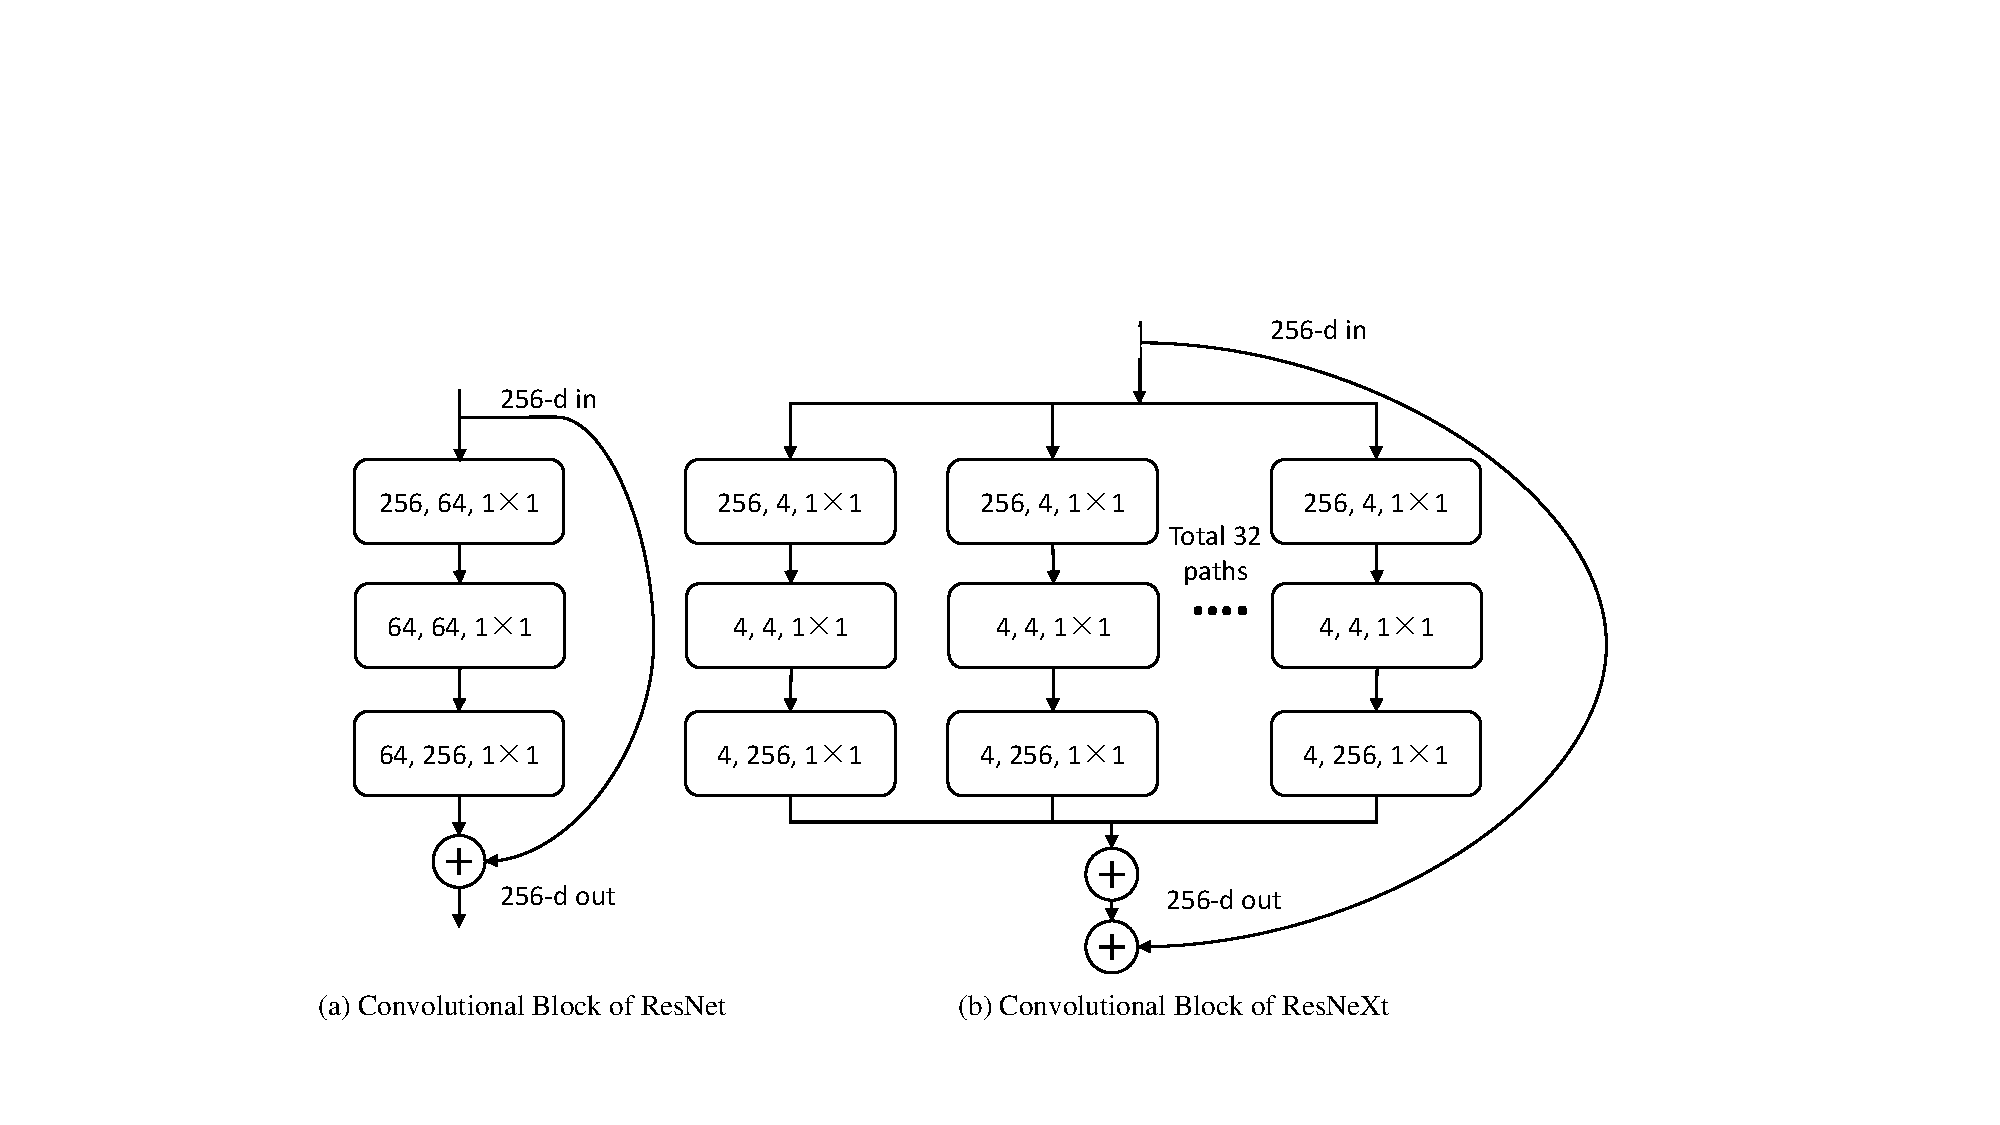
\includegraphics[width=1\textwidth]{figures/resnext}
\caption{Saliency maps by different configurations of the network. From left to right, they are saliency maps by only.}
\label{resnext}
%\vspace{-5pt}
\end{figure*}

在介绍ResNeXt之间,需要再说明一下ResNet网络,因为ResNeXt是由ResNet发展变化而来。ResNet众所周知,因为其结构的合理性,不仅在学术界影响深远,现在很多工业的方法都需要利用到这一网络。ResNet的核心就是旁路(shortcut),在主序网络的外面引入一条支路,保持前项网络顺利进行的同时,可以有效地解决由于网络过深所造成的梯度消失问题,进而使得深度网络层数据可以大大增加。例如,之前的VGGNet最高有19层,而ResNet可以把层数加到152。由于层数的增加,学习到的特征也就更为鲁棒,因此ResNet可以在多个任务上都取得成功。

ResNeXt是ResNet的改进,两者个对比如图\ref{resnext}所示,(a)为ResNet结构,而(b)ResNeXt为结构。为了简便与直观,图中只展示了两个网络中的一个卷积块(block),卷积块的输入都是通道数为256的特征图,而输出也同样为256。从图中可以明显地看出ResNeXt比ResNet要宽,ResNeXt把原来ResNet只需要一个卷积处理的特征图,分配到多个卷积支路中,最后再由一个求和操作合并,这样结构称之为Inception。Inception结构是通过多个卷积核得到不同的特征图,这样我们可以得到多样性的特征,可以理解为当我们观察一个物体时,我们可以从不同的视角、距离去``看"目标。

整个ResNeXt网络就是由改进过的卷积残差块堆叠而成,所以ResNeXt也可以通过增加或减少残差块来控制网络的深度,根据不同的需要构建不同的ResNeXt网络,比较常用的有ResNeXt-50、ResNeXt-101、ResNeXt-152等。本文的基础网络使用到的就是ResNeXt-101。

\subsection{ASPP结构}
ASPP结构是本文引入的另一个重要模块。该模块是在文献\cite{chen2017rethinking}提出,主要是用来解决图像分割问题的方法。由于显著性目标检测和图像分割在任务中存在一定的相似性,所以ASPP结构也逐渐被引入显著检测的网络结构。深度网络的成功关键在于其可以把图像充分的抽象,并在抽象化后可以有效的保持图像的内在不变性。然而,这种不变性在高层语义提取中很难保持空间信息不变。因为,高层的语义需要使用pooling层不断把特征图尺度减小,进而破坏掉图像原有的空间信息。ASPP就是希望找到一个平衡点,同时完成语义的抽象和保持空间信息不变。具体实现是:

首先,ASPP在整个网络中减少pooling层的数量,从而使特征图的尺度保持在一个合适的范围,同时引入膨胀卷积,并通过调整不同的膨胀系数,增加卷积操作的感受野,进而学习到鲁棒的空间上下文信息。因此,ASPP可以看做是一个由不同参数的膨胀卷积组合而成的空间特征学习模块。

\begin{figure*}
%\vspace{-100pt}
\center
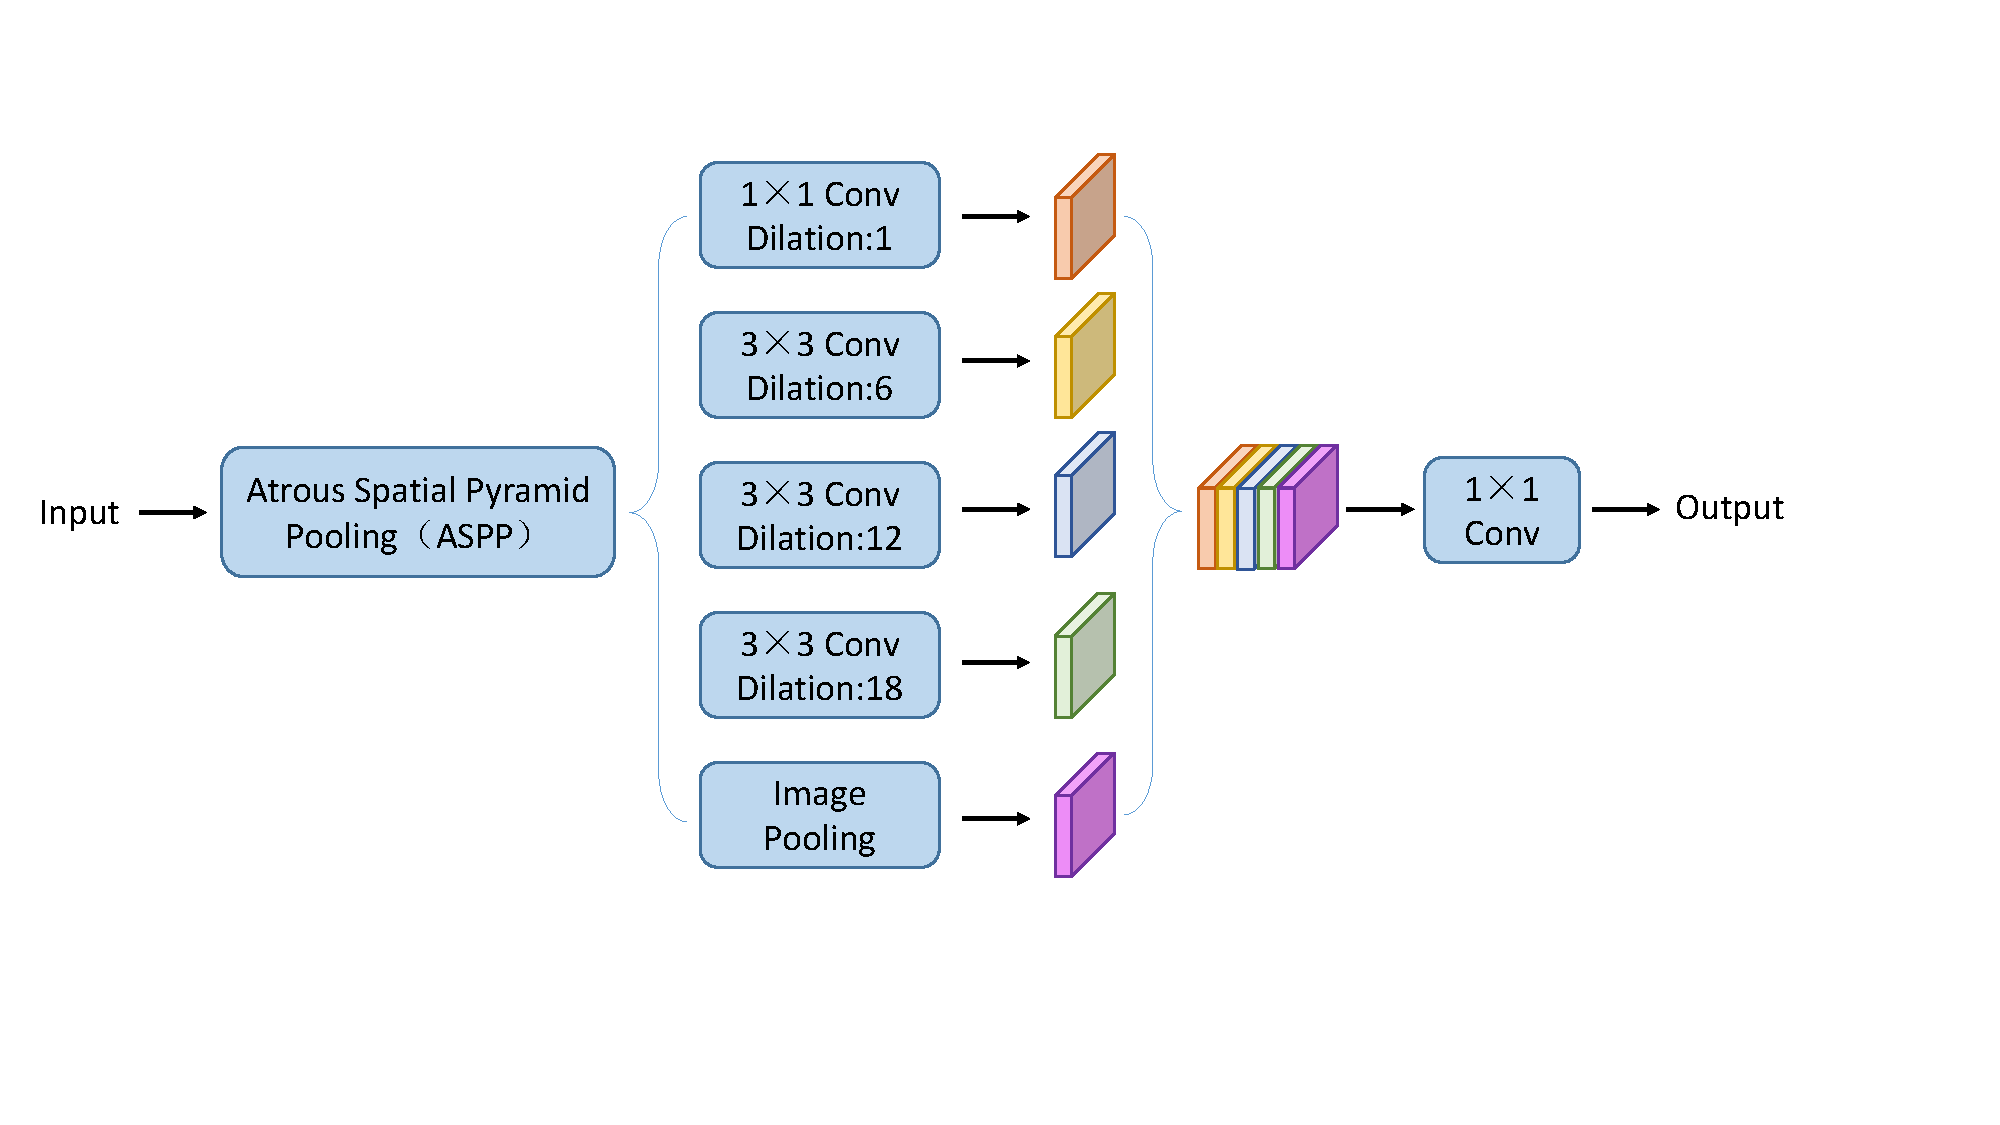
\includegraphics[width=1\textwidth]{figures/aspp}
\caption{Saliency maps by different configurations of the network. From left to right, they are saliency maps by only.}
\label{aspp}
%\vspace{-5pt}
\end{figure*}

其次,提出空间卷积池化金字塔。ASPP结构即是一个空间金字塔结构,金字塔中不同的层即由不同参数的膨胀卷积表示,具体的结构可在图\ref{aspp}可以看到,图中共有5个不同的金字塔层,其中4层为膨胀卷积,膨胀系数分别为1、6、12、18;第5层是一个直接图像pooling层;这5层生成的特征图使用Concat操作堆叠,然后再采用一个卷积核为1$\times$1的卷积进行融合,作为ASPP模块的特征图输出,供其他模块使用。空间金字塔的目的就是为了用不同尺度的感觉野对特征图进行探测,以不同的比例检测目标,同时提取特征图的空间上下文信息。

\section{方法描述}
本章提出的帧间运动增强网络包括四个部分。首先是基础网络,主要完成静态显著特征的提取,由于ResNeXt和空间金字塔池化模块(ASPP)组成。其次是初始运动特征提取,本文采用一个循环(recurrent)结构进行初步的运动特征提取。接着是帧间运动特征增强,通过使用前一个模块得到的特征图,利用帧间关系完成运动增强。最后,历史显著图引导,嵌入在运动特征增强模块中,利用前面预测出的显著图来引导当前帧的显著图的学习。给定一段原始的输入帧,通过基础网络获得静态的(空间上的)特征图,之后完成初始运动特征提取,接着通过帧间特征增强完成最后的视频显著性估计。

由于在上一小节中,本文已经详细介绍了本文基础网络的主要构成,因此,本节的内容主要是包括三个部分,初始运动特征提取、帧间运动特征增强和历史显著图引导。

\subsection{初始运动特征提取}
本章使用到的基础网络是由ResNeXt和ASPP结构组成,主要用于静态图像空间特征的提取。为了完成视频序列的显著性检测,运动特征需要被引入,因此,本文提出了一个两阶段的运动特征提取。本节首先介绍初始运动特征提取模块。

初始运动特征提取模块是一个循环结构(recurrent),可以引入任意一个循环网络结构,如RNN、LSTM、GRU等。又由于原始的RNN结构问题,其提取到的运动特征区分性较弱,所以本文验证了LSTM和GRU两种结构。LSTM结构在上一章中已有详细介绍,即通过各个限制门控制时序特征的学习。而GRU,全名是Gated recurrent units,由于属于RNN家族,因此输入和输出与LSTM是一样的,都是输入一组时序信息和初始化的内部隐层参数(一般初始化为零),输出则为学习到的隐层参数和对应序列特征,同时也可以调整输出层的结构得到不形式的输出,即多对一输出和多对多输出。相对于LSTM,GRU是为了应对计算资源不足情况和提高计算效率,其结构要相对简单。在LSTM中,其主要结构是三个控制们,分别是输入门、遗忘门和输出门。而GRU却只有两个门,一个是重置门(reset gate),另一个是更新门(update gate)。因此,GRU的计算方式可以归纳为:

\begin{equation}
\label{gru}
\begin{aligned}
   R_{t}  &= \sigma(W_{xr} * X_t + W_{hr} * H_{t-1} + b_r) \\
   Z_{t}  &= \sigma(W_{xz} * X_t + W_{hz} * H_{t-1} + b_z) \\
   \tilde{H_t} &= tanh(W_{x\tilde{h}} * X_t + R_{t} \circ W_{h\tilde{h}} * H_{t-1}  ) \\
   H_t &= (1 - Z_{t}) * H_{t-1} + Z_{t} * \tilde{H_t}
 \end{aligned}
\end{equation}

其中,$R_{t}$与$Z_{t}$即为重置门和更新门;$X_{t}$是GRU的输入,$t$表示当前状态;$H_{t-1}$是GRU的隐层参数,$t-1$表示前一状态;$W_{(\cdot)(\cdot)}$即为各个运算中待学习的网络参数。$b_{(\cdot)}$为偏置项;$\sigma(\cdot)$则sigmoid激活函数,与$tanh(\cdot)$一起把线性运算转化为非线性运算;由于本文任务是像素级分类,所以运动特征模块都是卷积运算,不是传统的全连接,$`*'$和$`\circ'$分别为卷积运算和哈达玛积。

可以看到,输入数据$X_{t}$,首先计算$R_{t}$与$Z_{t}$,然而再计算候选隐藏层$\tilde{H_t}$,这一个状态与LSTM中的$C_t$类似,可以看成对当前输入信息和前一状态信息的编码,并确定当前状态。其中,$R_{t}$用来保持之前的记忆,若$R_{t}$为零时,说明当前状态只由输入信息决定。之后,通过$Z_{t}$遗忘掉多余的隐藏层信息$H_{t-1}$,得到当前时刻的隐藏层,并作为输出和下一次迭代。

对比LSTM,GRU的结构相对简单,但是其结构也可以利用前一状态的信息来学习当前状态,因此GRU也可以很好地学习到运动信息信息。而且其运算效率也略高于LSTM,也更为实用训练数据较少的任务,视频显著性检测正符合这一条件。

\subsection{帧间运动特征增强}

\begin{figure*}
%\vspace{-100pt}
\center
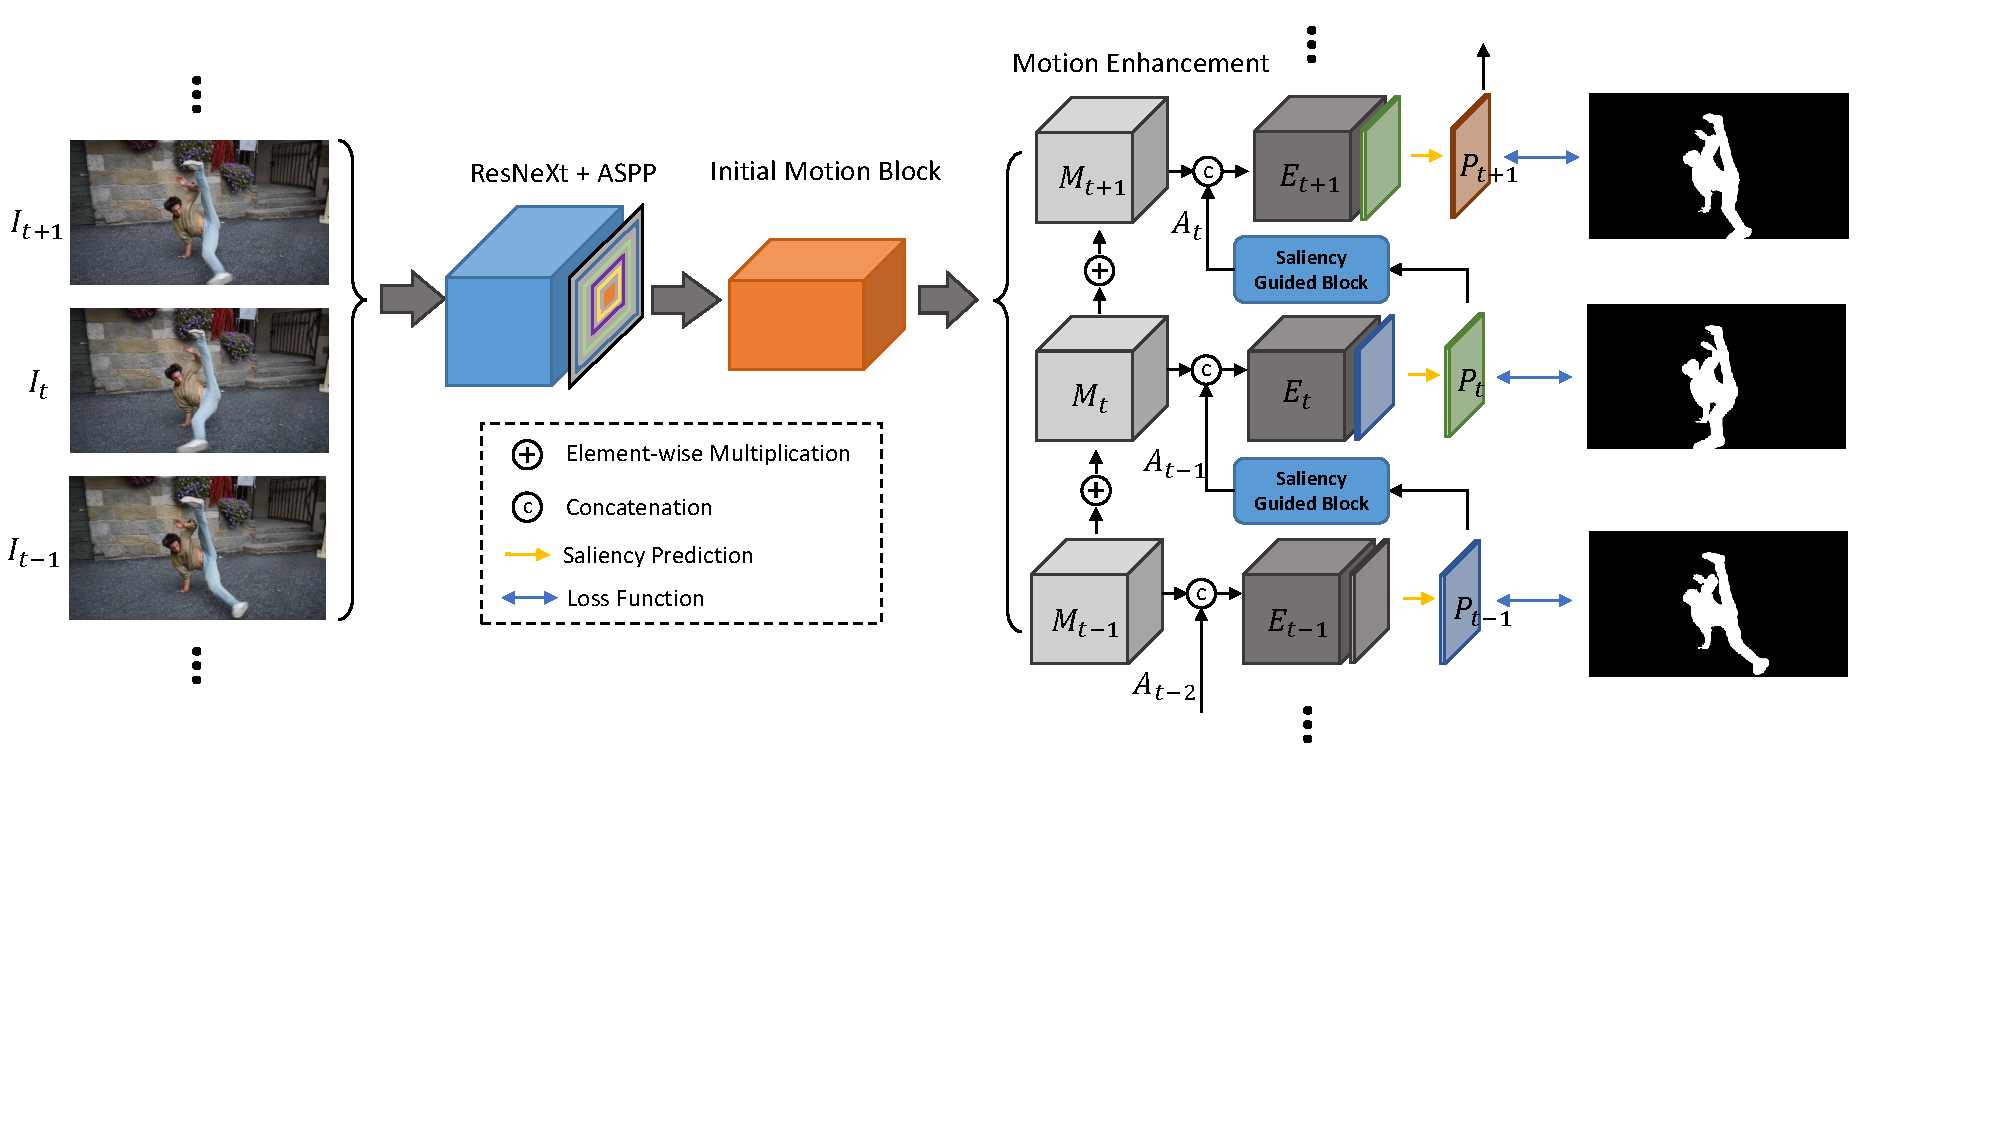
\includegraphics[width=1\textwidth]{figures/framework3}
\caption{Saliency maps by different configurations of the network. From left to right, they are saliency maps by only.}
\label{framework3}
%\vspace{-5pt}
\end{figure*}

两阶段提取运动特征的第二步是帧间运动特征增加。由于发现了一些复杂视频序列中存在两个连续帧差距较大的问题,所以为了解决这一现象,本文提出了这一个模块来增强运动特征。具体的做法如图\ref{framework3}所示,输入的视频序列$\{..., I_ {t-1}, I_{t}, I_{t}, ...\}$首先被送入ResNeXt和ASPP的卷积结构体提取视频帧内的静态空间特征。然而,再使用上一结所描述的初始运动特征提取模块获得初始运动特征图,即为图中的$\{..., M_{t-1}, M_{t}, M_{t}, ...\}$。之后,为了增大当前帧的特征图的内部数值,本文把前一帧的特征图,直接加到当前帧的特征图上,从而得到增强后的特征图$\{..., E_{t-1}, E_{t}, E_{t}, ...\}$。并且,由于特征图序列是不断的相加,理论上序列的最后一帧可以带上之前帧所有信息。最后增强后的特征图再堆叠一个显著性引导图$A_{t}$,通过一个显著性预测模块完成最后的显著性估计,得到最终的显著性预测结果$\{..., P_{t-1}, P_{t}, P_{t}, ...\}$。

在整个过程中,为了进一步加深对历史信息的学习,本文在帧间运动特征增强模块中嵌入了一个显著图引导结构。其主要利用之前估计出的显著图来引导当前帧显著性预测,这一模块的具体结构将在下一小节讨论。

我们可以总结帧间运动特征增强模块的所有计算为如下公式:

\begin{equation}
\label{gru}
\begin{aligned}
   P_{t}  &= \Gamma(Cat(M_{t-1} + M_{t}, A_{t-1});W_m) \\
   A_{t-1}  &= G(P_0, ..., P_{t-2};W_s); i \in \bm{N_{+}}
 \end{aligned}
\end{equation}

其中,$P_{t}$即为当前第t帧估计的显著图;$M_{t-1}$和$M_{t}$分别为前一帧和当前帧由初始运动模块提取到的特征图;$A_{t}$的显著图引导结构的输出,而$\{P_0, ..., P_{t-2}\}$则为之前帧的显著图;$\Gamma(\cdot;\cdot)$是显著性估计的一系列卷积操作,具体包括三个使用Batchnorm和PReLU激活的卷积层,前两层的卷积核是3$\times$3,最后一层是1$\times$1;而$G(\cdot;\cdot)$为显著图来引导操作;$W_{m}$和$W_{s}$分别对应它们各自的参数。

\subsection{显著图引导}

\begin{figure*}
\center
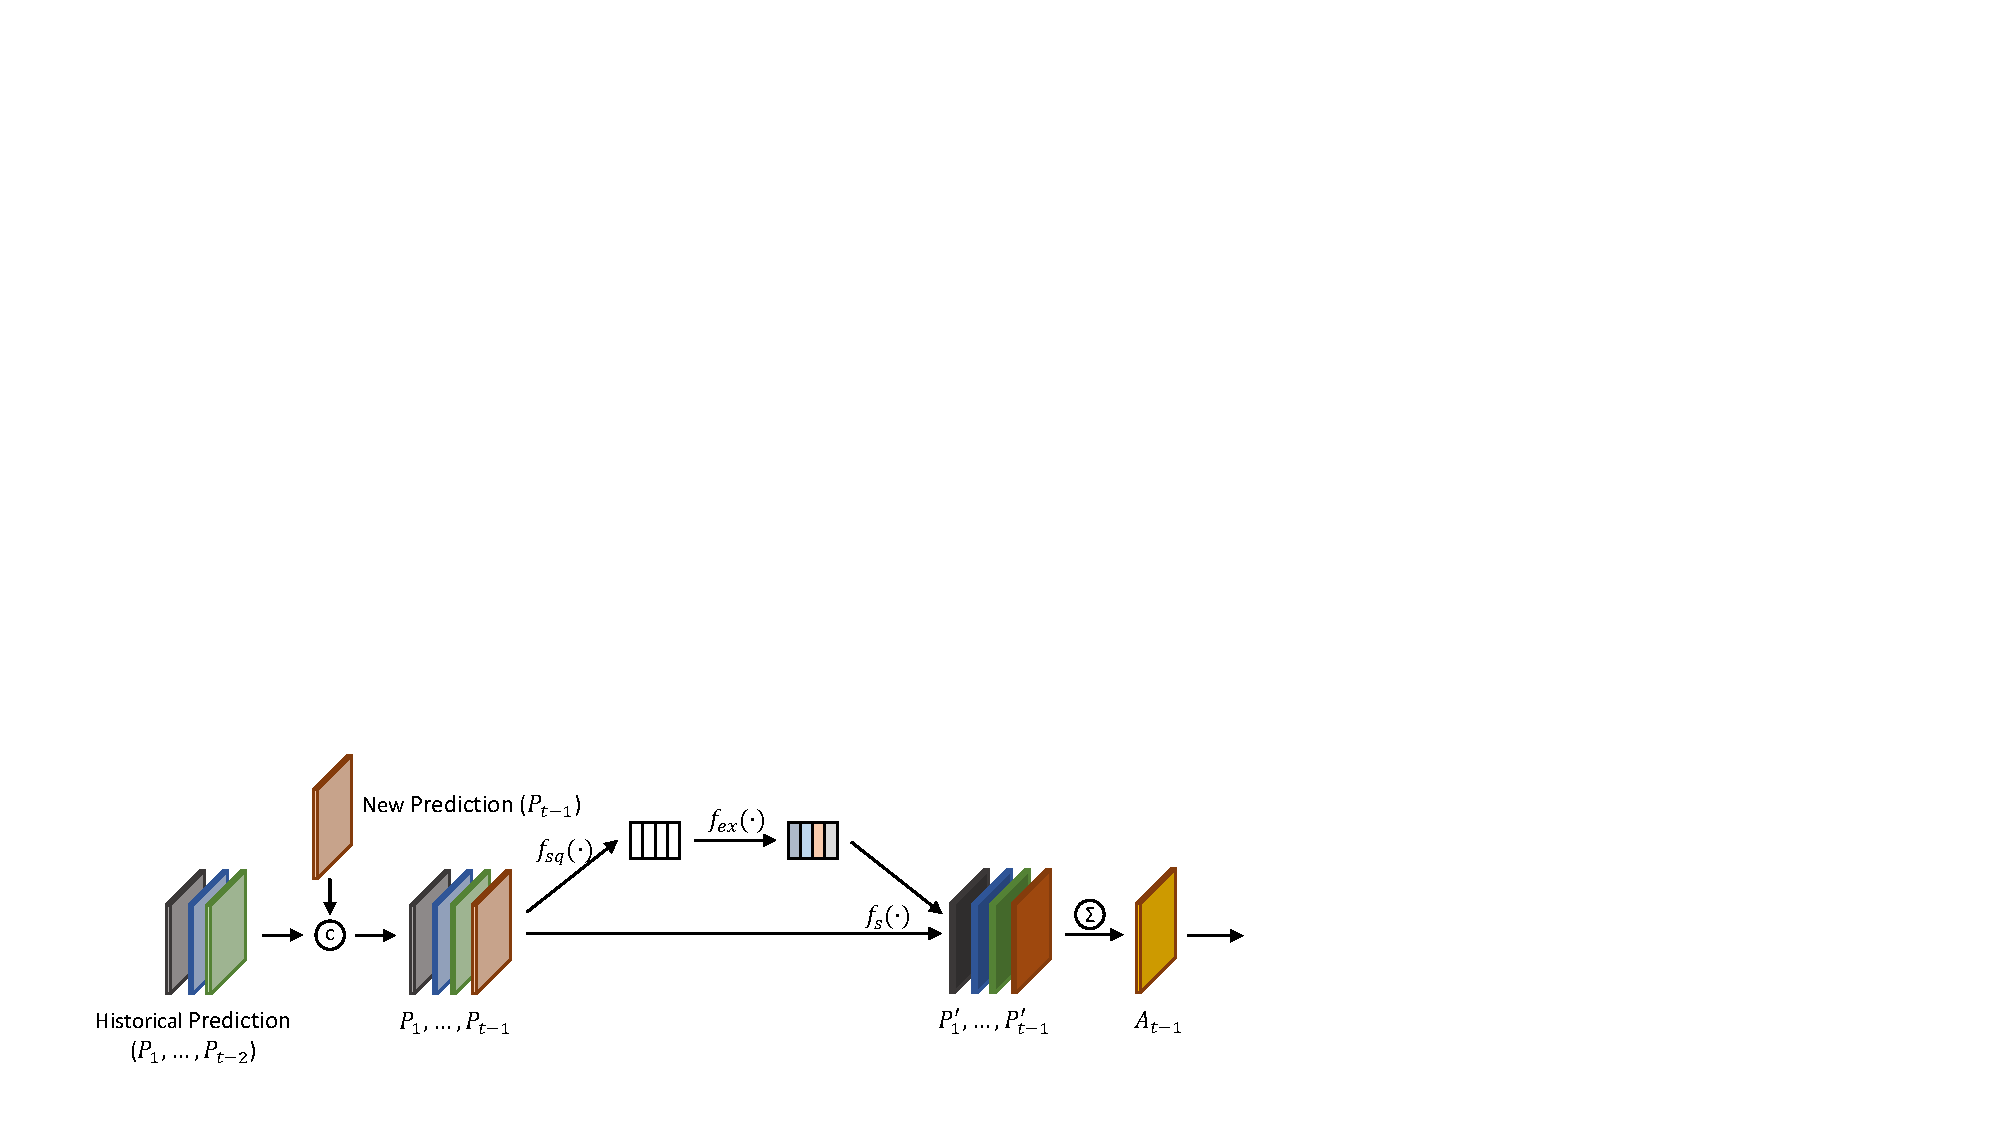
\includegraphics[width=1\textwidth]{figures/se}
\caption{Saliency maps by different configurations of the network. From left to right, they are saliency maps by only.}
\label{se}
%\vspace{-5pt}
\end{figure*}

为了辅助运动特征增强模块的特征学习和进一步增强运动特征,在增强模块中,本文加入了一个显著性引导结构。该模型是受文献\cite{wang2016saliency}和\cite{deng2018r3net}启发,前者开始是引入一个外部先验,然后再生成自己的显著图,并作为新的先验进行迭代学习。后者同样是一个循环结构,采用在网络的后端把显著图作为先验来学习网络。两篇论文在原理上都是类似的,都是使用显著先验引导网络学习,只是先验的来源不同。在视频显著性检测的任务中,这种先验引导的方法就特别适用。并且,为了充分利用历史信息,本文引入了一个显著图引导模块来存储之前帧生成的显著图,并采用一个压缩-激励机制(Squeeze-and-Excitation)来融合历史显著图,进而生成先验图引导当前帧增强运动特征。

本文的显著图引导的具体结构如图\ref{se}所示。从中我们可以看到,结构内部存储的历史显著性估计$\{P_1, ..., P_{t-2}\}$会先与新的预测堆叠$P_{i-1}$,然后进行空间压缩,利用一个全局平均池化把特征图压缩成1$\times$1的尺度,这一个过程可以归纳为:

\begin{equation}
\label{sq}
\begin{aligned}
   z_{c} =f_{sq}(P_c) = \frac{1}{H \times W} \sum\limits_{i=1}^{H} \sum\limits_{j=1}^{W} P_c; c &\in \{0,1,...,t-1\}
 \end{aligned}
\end{equation} 我们可以看到,公式\ref{sq}就是针对每一个历史特征图$P_{c}$进行平均池化,从而得到尺度为$R^C$(C为输入特征图的通道数)的特征值$z_{c}$。为了得到跨通道之间的非线性关系,学习非互斥信息,因此压缩后的特征值需要使用到一个两层全连接计算和相应的分线性激活函数。具体可以定义为$f_{ex}(\cdot)$操作:

\begin{equation}
\label{ex}
\begin{aligned}
   s = f_{ex}(\bm{z}, \textbf{W}) = \sigma(g(\bm{z}, \bm{W})) = \sigma(\bm{W_2}\delta(\bm{W_1}\bm{z}))
 \end{aligned}
\end{equation} 

其中,$\bm{z}$即为压缩过程中得到的特征向量;$\bm{W_1} \in R^{\frac{C}{r}\times C} $ 和$\bm{W_2} \in R^{C\times \frac{C}{r}} $分别是两个全连接层的参数,$r$是压缩比,用来调整特征维度和计算效率;$\delta(\cdot)$和$\sigma(\cdot)$是两个激活函数,分别是sigmoid和ReLU。在获得特征图的权重$s$后,需要给原有的特征图乘上这一个权值,进行$f_s(\cdot)$操作:

\begin{equation}
\label{scale}
\begin{aligned}
   \bm{\tilde{P}_c} = f_{s}(\bm{P}_c, s_c) = s_c \cdot \textbf{P}_c
\end{aligned}
\end{equation} $f_s(\cdot)$操作很好理解,就是给原有个特征图,这里是历史显著图$\bm{P}_c$乘上之前学习到的权值$s_c$,最终得到加权后的特征图$\bm{\tilde{P}}_c$。

最后,本文需要把所有的历史显著图融合成一个先验图来引导后一帧的运动特征学习,因此我们在显著性引导的最后加入了一个求和操作,即用对应位置相加的方法:
\begin{equation}
\label{sum_scale}
\begin{aligned}
   A_i = \sum\limits_{c=1}^{t-1}\tilde{P}_c
 \end{aligned}
\end{equation} $A_i$即为显著图引导模块最后的输出先验图,在图\ref{framework3}也可以看到,$A_i$会与后一帧得到的增强后运动特征$M_{i+1}$结合去预测后一帧的显著图$P_{i+1}$。


\section{实验结果和分析}

为了验证本章模型在视频显著性目标检测和视频分割上的有效性,本章首先介绍两组评价标准,分别对应两个任务;其次,介绍本章实验使用到的数据集。接着,给出帧间运动增强网络的具体实现;之后,分别在两套指标下对比相应的其他模型;最后,验证本章方法中各个模块的有效性。
\subsection{实验评价准则}
为了验证显著性检测与视频分割两个任务,本章共使用的两组评价准则。其一仍与上两章相同,使用PR曲线和平均绝对误差(MAE)。同时,本章又引入了新的评价方法F-measure,其可定义为:
\begin{equation}
\label{f_measure}
\begin{aligned}
   F_\beta = \frac{(1+\beta^2)Precision \times Recall }{\beta^2\times Precision + Recall}
 \end{aligned}
\end{equation} 其中,Precision与Recall是通过求显著图的平均值得到;$\beta^2$被设定为0.3用以平衡recision与Recall。

第二组评价标准则主要与视频分割相关,有三个评价准则:区域相似性(region similarity)、轮廓准确性(contour accuracy)、时序稳定性(temporal stability)。

区域相似性(J)是基于区域的分割相似度测量,它可以通过一定数量的错误标签提供直观且尺度不变的信息,其定义可以用下列公式表示:
\begin{equation}
\label{region_similarity}
\begin{aligned}
   J = \frac{\|M \cap G\|}{\|M \cup G\|}
 \end{aligned}
\end{equation} 其中,$M$和$G$分别表示算法分割结果和与之对应的真值(Ground Truth)。

轮廓准确性(F)是从轮廓的角度分析,可以将分割结果图$M$视为一组闭合的轮廓$c(M)$,它们限定了掩模的空间范围。因此,它可以计算轮廓空间里面的所有像素点的准确率和召回率。其公式定义为:
\begin{equation}
\label{region_similarity}
\begin{aligned}
   F = \frac{2P_cR_c}{P_c + R_c}
 \end{aligned}
\end{equation} 其中,$P_c$和$R_c$即为轮廓区域里面的像素点准确率与召回率。

时序稳定性(T),直观上来看,区域相似性表示的是分割结果的每个像素点是否匹配,而轮廓准确性则表达的是其轮廓上的准确率性,时序稳定性则表示的是时间维度上的相关信息,因为分割目标有可能随着时间的推移会存在一定的形变。其原理是最小化形状上下文描述子(Shape Context Descriptor)来实现。具体的计算公式参考文献[Dynamic Time Warping (DTW)]。
\subsection{数据集}
本章一共使用到了7个数据集,分别是DUT-OMRON、FBMS、DAVIS、SegTrack-V2、MCL、VOS。其中DUT-OMRON和DAVIS的30个序列用于网络训练,FBMS的测试集、DAVIS余下的20个序列、SegTrack-V2、MCL和VOS用于验证本章提出的深度方法。在上述数据集中,DUT-OMRON是图像显著性检测的数据集,共5168张图像;其余都是视频显著性检测数据集,其中FBMS有720帧标签,DAVIS有3455帧标签,SegTrack-V2有1065帧标签,MCL共463帧标签,VOS共7467帧标签。

\subsection{实现细节}
本章的帧间运动特征增强网络在实现时需要注意几个细节:

首先,最终的网络参数是通过两段学习得到。第一阶段训练使用的是图像数据(即DUT-OMRON)和DAVIS中的视频帧,同时网络是BaseLine网络,没有嵌入运动特征的学习。第二阶段使用的是视频序列训练,即DAVIS序列,并且以BaseLine网络参数作初始化,加入初始运动提取模块和帧间运动增强模块训练。

其次,基础网络是DeeplabV3的改进,加入了对多尺度特征嵌入,具体做法参考了R3Net,把ResNeXt的前三个卷积块作为一个组,提取低阶特征;后两个卷积块为另一个组提取高阶特征,之后采用一个循环结构对两组特征进行融合。

最后,帧间运动特征增强网络使用的优化算法是梯度下降(SGD),两段训练的学习率分别为$10^{-3}$和$10^{-5}$;权衰量为$5 \times 10^{-4}$;动量分别是0.9和0.95;BaseLine网络的初始化使用的是ImageNet的初始化参数。

\subsection{结果D}
\Blindtext

\section{讨论}
\Blindtext

\section{小结}
\Blindtext 